% ============================================================
%  Altar Valley Berms — Figure Summary  (Paper 2)
%  Paper 2: Distinguishing Breaches from Flanks
%  Captions drawn from figures/paper2/figure_registry_concise.txt
%  Date: 2026-03-01
% ============================================================
\documentclass[11pt, a4paper]{article}

\usepackage[utf8]{inputenc}
\usepackage[T1]{fontenc}
\usepackage{lmodern}
\usepackage[left=2.5cm, right=2.5cm, top=2.5cm, bottom=2.5cm]{geometry}
\usepackage{graphicx}
\usepackage{caption}
\usepackage{float}
\usepackage{parskip}
\usepackage{microtype}
\usepackage{hyperref}
\hypersetup{colorlinks=true, linkcolor=black, urlcolor=blue}

% ── compact figure caption style ─────────────────────────────
\captionsetup{font=small, labelfont=bf, justification=raggedright, singlelinecheck=false}

% ============================================================
\begin{document}

\begin{center}
  {\LARGE \textbf{Altar Valley Berms:}} \\
  {\LARGE \textbf{Distinguishing Breaches from Flanks}} \\[0.4em]
  {\large Figure Summary — Paper 2} \\[0.3em]
  {\small Generated 2026-03-01 \quad|\quad Source: \texttt{figures/paper2/figure\_registry\_concise.txt}}
\end{center}

\vspace{1em}
\hrule
\vspace{1.5em}

% ── Figure 2 ─────────────────────────────────────────────────
\begin{figure}[H]
  \centering
  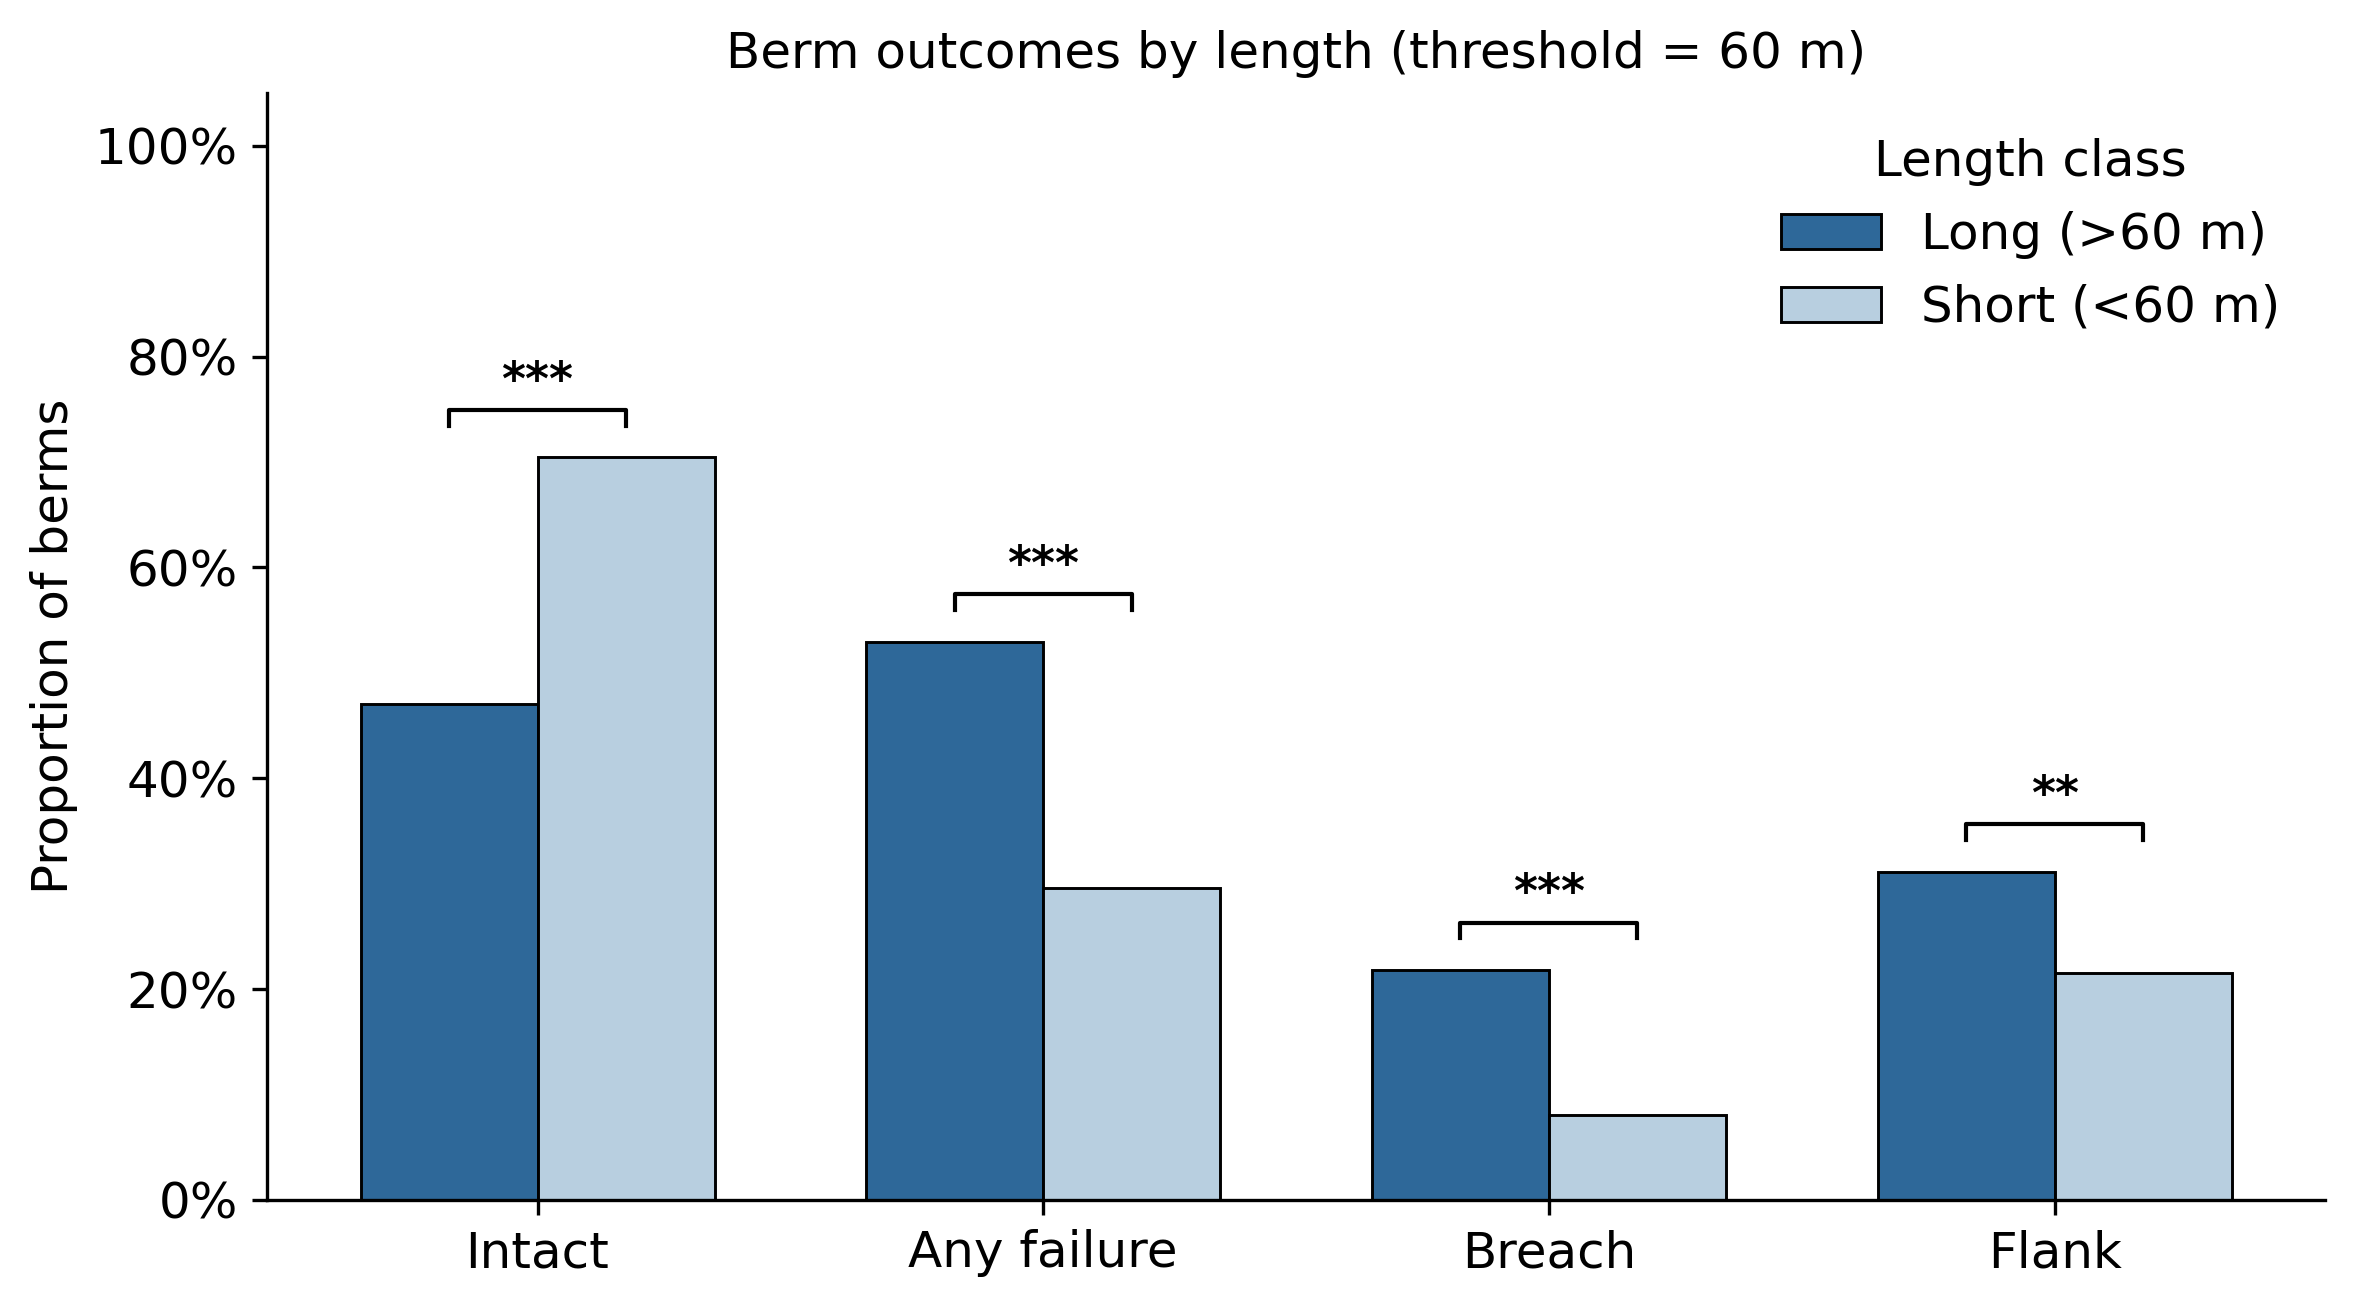
\includegraphics[width=\linewidth]{../figures/paper2/fig2.png}
  \caption*{\textbf{Figure 2.}
    Grouped comparison of berm outcome proportions between Long and Short berm
    classes, with per-metric 2$\times$2 contingency-table significance tests
    shown as bracket annotations.
    Outcome proportions differ by length class, and this figure serves as Paper~2
    Figure~2 for the breach/flank-focused comparison.}
\end{figure}

\end{document}
